\chapter{L'architettura proposta} % 4

Questo capitolo ha l'obiettivo di presentare l'architettura proposta per risolvere il problema affrontato dalla tesi. Prima verrà mostrata l'architettura generale, utilizzando un diagramma UML dei componenti e successivamente, per ciascun componente verranno individuate le responsabilità principali e le funzionalità. Infine, per chiarificare, sarà descritto un flusso di esecuzione completo, descrivendo ciò che succede partendo dall'inizio e arrivando fino alla fine.

\section{Architettura del sistema} % 4.1

Sto realizzando una tesi triennale sperimentale sull'argomento "Generazione automatica di moduli per l'intercettazione delle comunicazioni Command-and-Control dei malware".

Descrizione software: esegue il reverse engineering di malware Mirai attraverso agenti LLM, per poi generare il codice di intercettazione dei comandi ricevuti dal C2 server.

Adesso devo redigere la parte di progettazione dell'architettura del software.

All'interno di questo capitolo dovrò parlare dell'architettura complessiva del sistema e un po' più nello specifico dei singolo moduli, con le funzionalità che mi aspetto. Alla fine il contenuto di questo capitolo riguarda l'ingegneria del software e spiegare un po' le scelte e il flow.

Il nostro obiettivo sarà quello di capire come strutturare il capitolo e la relazione con quello successivo di implementazione.

\section{Idea di architettura}

Componenti:

\begin{itemize}
    \item Sistema di classificazione: malevolo + famiglia
    \item Agente di reverse engineering del codice
    \item Agente di generazione del codice di intercettazione
    \item Ghidra MCP
    \item Sandbox MCP
    \item Ghidra R.E.
\end{itemize}

Artefatti:

\begin{itemize}
    \item (input) file ignoto
    \item (input) knowledge base di conoscenza
    \item (output/input) file risultato di analisi: report + evidence
    \item (input) schema JSON parsing comandi
    \item (input) template codice
    \item (output) logging più o meno esteso
    \item (output) codice di intercettazione generato
    \item (input) prompt ?
\end{itemize}

Diagramma dei componenti 1: contiene delle aree evidenziate.

\iffalse
flowchart TD

%% =========================
%% Definizione Stili
%% =========================
classDef agent fill:#f9d0c4,stroke:#c0392b,stroke-width:2px,color:#333;
classDef mcp fill:#d4e6f1,stroke:#2980b9,stroke-width:2px,color:#333;
classDef tool fill:#fcf3cf,stroke:#f1c40f,stroke-width:2px,color:#333;
classDef io fill:#e8f8f5,stroke:#1abc9c,stroke-width:2px,color:#333;

%% =========================
%% Artefatti di Input / Output
%% =========================
Bin([File Binario Ignoto]):::io
KB[(Knowledge Base<br/>e System Prompts)]:::io
Templ[(Template Codice)]:::io
Logs[(Log di Tracciabilità)]:::io
Output([Codice di Intercettazione]):::io

%% =========================
%% Layer 1: Pipeline degli Agenti
%% =========================
subgraph Pipeline_Agenti["Pipeline di Analisi LLM"]
    Classifier["Modulo di Classificazione<br/>Triage"]:::agent
    REAgent["Agente di Reverse Engineering<br/>LLM-based"]:::agent
    GenAgent["Agente di Generazione Codice<br/>LLM-based"]:::agent
end

%% =========================
%% Layer 2: Modulo MCP
%% =========================
subgraph Layer_MCP["Model Context Protocol Layer"]
    GhidraMCP["Ghidra MCP<br/>Server"]:::mcp
    SandboxMCP["Sandbox MCP<br/>Server"]:::mcp
end

%% =========================
%% Layer 3: Strumenti Esecutivi
%% =========================
subgraph Strumenti["Ambienti di Esecuzione"]
    GhidraTool["Ghidra R.E.<br/>Headless"]:::tool
    SandboxEnv["Sandbox<br/>Dinamica"]:::tool
end

%% =========================
%% Artefatti Intermedi
%% =========================
Report[(Report & Evidenze<br/>JSON Schema C2)]:::io

%% =========================
%% Flusso Principale dei Dati
%% =========================
Bin --> Classifier
Classifier -->|"Conferma: Famiglia Mirai"| REAgent
REAgent -->|"Evidenze Estratte"| Report
Report --> GenAgent
GenAgent --> Output

%% =========================
%% Contesto agli Agenti
%% =========================
KB -.->|"Contesto / Regole"| REAgent
KB -.->|"Contesto / Regole"| GenAgent
Templ -.->|"Struttura Base"| GenAgent

%% =========================
%% Logging
%% =========================
Pipeline_Agenti -.-> Logs

%% =========================
%% Agenti <-> MCP
%% =========================
REAgent ==>|"Richiesta Tool<br/>(Decompile, Sys call, ecc.)"| GhidraMCP
REAgent ==>|"Richiesta Tool<br/>(Esegui, Sniff)"| SandboxMCP

%% =========================
%% MCP <-> Strumenti
%% =========================
GhidraMCP <--> |"API / Bridge"| GhidraTool
SandboxMCP <--> |"API / Bridge"| SandboxEnv
\fi 

Diagramma dei componenti 2: contiene tutti i componenti, input e output.

\iffalse
flowchart TD
%% Definizione Stili
classDef agent fill:#f9d0c4,stroke:#c0392b,stroke-width:2px,color:#333;
classDef mcp fill:#d4e6f1,stroke:#2980b9,stroke-width:2px,color:#333;
classDef tool fill:#fcf3cf,stroke:#f1c40f,stroke-width:2px,color:#333;
classDef io fill:#e8f8f5,stroke:#1abc9c,stroke-width:2px,color:#333;
classDef llm fill:#ffecd2,stroke:#8e44ad,stroke-width:2px,color:#333;
classDef primary fill:#e8daef,stroke:#ff7f50,stroke-width:3px,color:#333;

%% Artefatti di I/O
Bin([File Binario Ignoto]):::primary
KB[(Knowledge Base)]:::io
Prompts[(Istruzioni e Prompt)]:::io
Templ[(Template Codice)]:::io
JSONSchema[(Schema JSON\nComandi C2)]:::io
Report[(Report & Evidenze)]:::io
Logs[(Log di Tracciabilità)]:::io
Output([Codice Python\nIntercettazione]):::primary
Halt([Termine Pipeline]):::io

%% Componente LLM
LLM[Large Language Model]:::llm

%% Pipeline Agenti e MCP Clients
Classifier[Modulo di Classificazione]:::agent

RE_Core[Logica Agente RE]:::agent
SRE_Client[SRE MCP Client]:::mcp
SandboxClient[Sandbox MCP Client]:::mcp

GenAgent[Agente di Generazione Codice]:::agent

%% Layer MCP Server
SRE_MCP[Framework SRE\nMCP Server]:::mcp
SandboxMCP[Sandbox\nMCP Server]:::mcp

%% Strumenti Esecutivi
subgraph Strumenti [Ambienti di Esecuzione]
    SRE_Tool[Framework SRE]:::tool
    SandboxEnv[Sandbox Dinamica]:::tool
end

%% Flusso Dati Principale
Bin --> Classifier
Classifier -- "Malevolo" --> RE_Core
Classifier -. "Non Malevolo: Stop" .-> Halt

RE_Core -- "Estrazione" --> Report
Report --> GenAgent
GenAgent --> Output

%% Flusso Prompt e KB
Prompts -. "Contesto/Regole" .-> RE_Core
Prompts -. "Contesto/Regole" .-> GenAgent
KB -. "Riferimenti (Opzionale)" .-> RE_Core

%% Connessioni LLM
RE_Core <--> |"Reversing/Reasoning"| LLM
GenAgent <--> |"Code Gen"| LLM

%% Connessioni MCP: Separazione Call / Result (Agent <-> Client)
RE_Core -- "Tool Call" --> SRE_Client
SRE_Client -- "Tool Result" --> RE_Core

RE_Core -- "Tool Call" --> SandboxClient
SandboxClient -- "Tool Result" --> RE_Core

%% Connessioni MCP: Trasporto (Client <-> Server)
SRE_Client <--> |"stdio / HTTP"| SRE_MCP
SandboxClient <--> |"stdio / HTTP"| SandboxMCP

%% Connessioni Server -> Strumenti
SRE_MCP <--> |"Bridge / API"| SRE_Tool
SandboxMCP <--> |"Bridge / API"| SandboxEnv

%% Input per la Generazione e Logging
Templ -. "Struttura Base" .-> GenAgent
JSONSchema -. "Mappatura" .-> GenAgent
RE_Core -.-> Logs
\fi

Diagramma di sequenza MCP:

\iffalse
sequenceDiagram
participant LLM
participant SREAgent as SRE Agent

participant SandboxMCPClient as Sandbox MCP Client
participant SandboxMCPServer as Sandbox MCP Server
participant SandboxExecutionEnvironment as Sandbox Execution Environment

participant SREFrameworkMCPClient as SRE Framework MCP Client
participant SREFrameworkMCPServer as SRE Framework MCP Server
participant SREFrameworkExecutionEnvironment as SRE Framework Execution Environment

rect rgb(245, 245, 245)
    Note over SREAgent, SREFrameworkMCPServer: Initialization
    SREAgent->>SandboxMCPClient: Create MCP client instance
    SREAgent->>SREFrameworkMCPClient: Create MCP client instance
    SandboxMCPClient->>SandboxMCPServer: Initialize/connect MCP server
    SREFrameworkMCPClient->>SREFrameworkMCPServer: Initialize/connect MCP server
end

rect rgb(235, 245, 255)
    Note over LLM, SandboxExecutionEnvironment: list_tools flow
    LLM->>SandboxMCPClient: list_tools
    SandboxMCPClient->>SandboxMCPServer: Request tool list
    SandboxMCPServer-->>SandboxMCPClient: Return tool list
    SandboxMCPClient-->>LLM: list_tools response
end

Note over LLM, SREFrameworkExecutionEnvironment: Time passes and other actions occur

rect rgb(235, 255, 235)
    Note over LLM, SREFrameworkExecutionEnvironment: call_tools flow
    LLM->>SREFrameworkMCPClient: call_tools(name: string, arguments: dictionary)
    SREFrameworkMCPClient->>SREFrameworkMCPServer: Call tool(name: string, arguments: dictionary)
    SREFrameworkMCPServer->>SREFrameworkExecutionEnvironment: Execute tool(name: string, arguments: dictionary)
    SREFrameworkExecutionEnvironment-->>SREFrameworkMCPServer: Return execution result
    SREFrameworkMCPServer-->>SREFrameworkMCPClient: Return call result
    SREFrameworkMCPClient-->>LLM: call_tools response
end
\fi

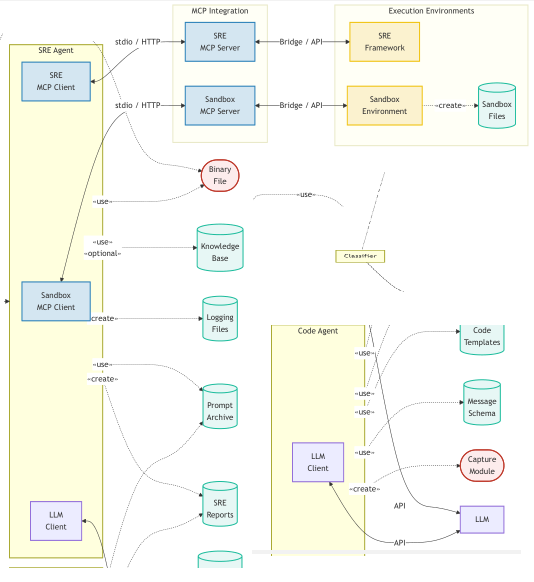
\includegraphics[scale=.4]{img/componenti.png}

\hspace{1cm}

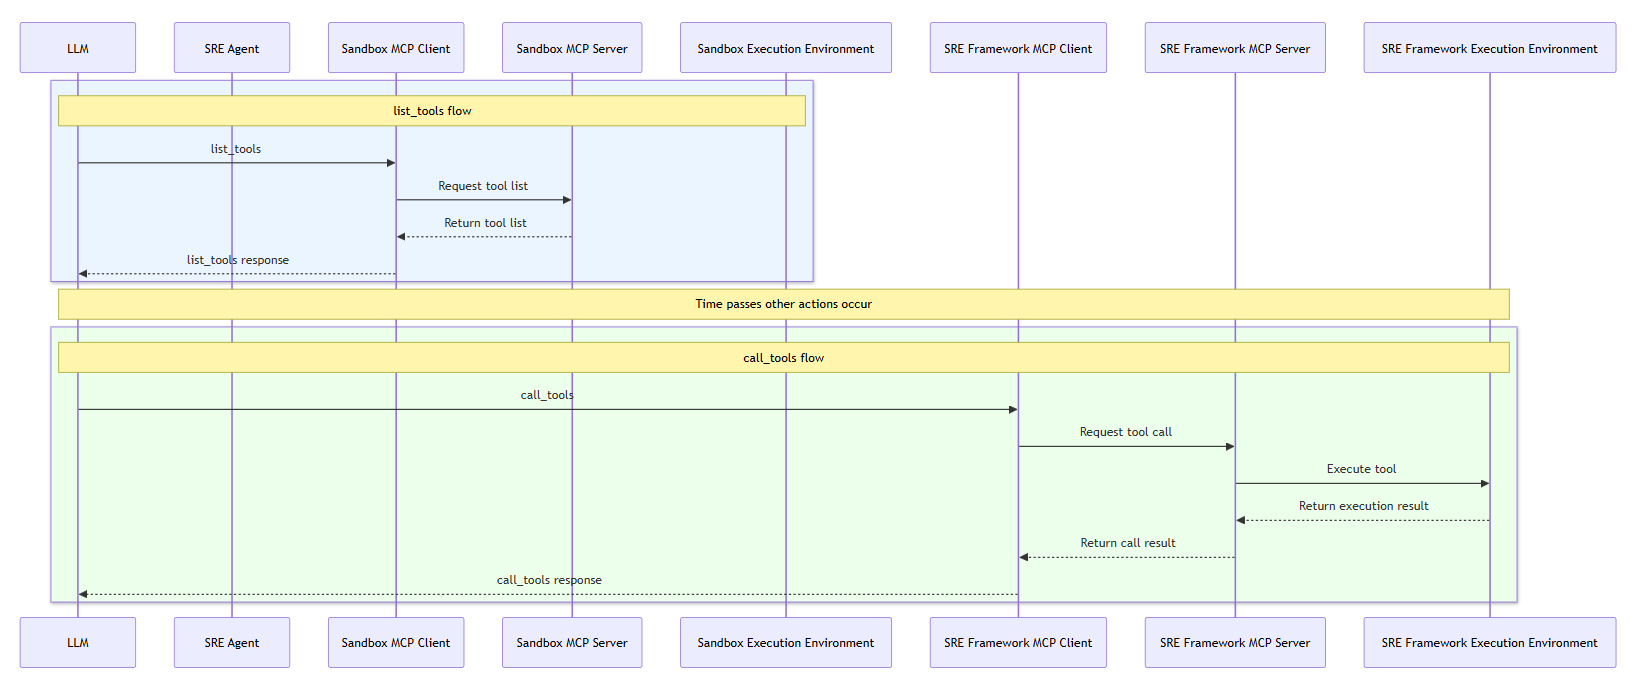
\includegraphics[scale=.4]{img/sequenza.png}